% Für Bindekorrektur als optionales Argument "BCORfaktormitmaßeinheit", dann
% sieht auch Option "twoside" vernünftig aus
% Näheres zu "scrartcl" bzw. "scrreprt" und "scrbook" siehe KOMA-Skript Doku
\documentclass[12pt,a4paper,headinclude,bibtotoc]{scrartcl}


%---- Allgemeine Layout Einstellungen ------------------------------------------

% Für Kopf und Fußzeilen, siehe auch KOMA-Skript Doku
\usepackage[komastyle]{scrpage2}
\pagestyle{scrheadings}
\automark[section]{chapter}
\setheadsepline{0.5pt}[\color{black}]

%keine Einrückung
\parindent0pt

%Einstellungen für Figuren- und Tabellenbeschriftungen
\setkomafont{captionlabel}{\sffamily\bfseries}
\setcapindent{0em}

\usepackage{caption}

%---- Weitere Pakete -----------------------------------------------------------
% Die Pakete sind alle in der TeX Live Distribution enthalten. Wichtige Adressen
% www.ctan.org, www.dante.de

% Sprachunterstützung
\usepackage[ngerman]{babel}

% Benutzung von Umlauten direkt im Text
% entweder "latin1" oder "utf8"
\usepackage[utf8]{inputenc}

% Pakete mit Mathesymbolen und zur Beseitigung von Schwächen der Mathe-Umgebung
\usepackage{latexsym,exscale,amssymb,amsmath}

% Weitere Symbole
\usepackage[nointegrals]{wasysym}
\usepackage{eurosym}

% Anderes Literaturverzeichnisformat
%\usepackage[square,sort&compress]{natbib}

% Für Farbe
\usepackage{color}

% Zur Graphikausgabe
%Beipiel: \includegraphics[width=\textwidth]{grafik.png}
\usepackage{graphicx}

% Text umfließt Graphiken und Tabellen
% Beispiel:
% \begin{wrapfigure}[Zeilenanzahl]{"l" oder "r"}{breite}
%   \centering
%   \includegraphics[width=...]{grafik}
%   \caption{Beschriftung} 
%   \label{fig:grafik}
% \end{wrapfigure}
\usepackage{wrapfig}

% Mehrere Abbildungen nebeneinander
% Beispiel:
% \begin{figure}[htb]
%   \centering
%   \subfigure[Beschriftung 1\label{fig:label1}]
%   {\includegraphics[width=0.49\textwidth]{grafik1}}
%   \hfill
%   \subfigure[Beschriftung 2\label{fig:label2}]
%   {\includegraphics[width=0.49\textwidth]{grafik2}}
%   \caption{Beschriftung allgemein}
%   \label{fig:label-gesamt}
% \end{figure}
\usepackage{subfigure}
\usepackage{adjustbox}

% Caption neben Abbildung
% Beispiel:
% \sidecaptionvpos{figure}{"c" oder "t" oder "b"}
% \begin{SCfigure}[rel. Breite (normalerweise = 1)][hbt]
%   \centering
%   \includegraphics[width=0.5\textwidth]{grafik.png}
%   \caption{Beschreibung}
%   \label{fig:}
% \end{SCfigure}
\usepackage{sidecap}

% Befehl für "Entspricht"-Zeichen
\newcommand{\corresponds}{\ensuremath{\mathrel{\widehat{=}}}}

%Für chemische Formeln (von www.dante.de)
%% Anpassung an LaTeX(2e) von Bernd Raichle
\makeatletter
\DeclareRobustCommand{\chemical}[1]{%
  {\(\m@th
   \edef\resetfontdimens{\noexpand\)%
       \fontdimen16\textfont2=\the\fontdimen16\textfont2
       \fontdimen17\textfont2=\the\fontdimen17\textfont2\relax}%
   \fontdimen16\textfont2=2.7pt \fontdimen17\textfont2=2.7pt
   \mathrm{#1}%
   \resetfontdimens}}
\makeatother

%Si Einheiten
\usepackage{siunitx}

%c++ Code einbinden
\usepackage{listings}
\lstset{numbers=left, numberstyle=\tiny, numbersep=5pt}

%Differential
\newcommand{\dif}{\ensuremath{\mathrm{d}}}

%Boxen,etc.
\usepackage{fancybox}
\usepackage{empheq}

%Fußnoten auf gleiche Seite
\interfootnotelinepenalty=1000

%Dateien aus Unterverzeichnissen
\usepackage{import}

%Bibliography \bibliography{literatur} und \cite{gerthsen}
%\usepackage{cite}
\usepackage{babelbib}
\selectbiblanguage{ngerman}

\begin{document}

\title{Flattern}
\author{Felix Kurtz}
\maketitle

\section{Einleitung}
Flattern ist ein unerwünschter aeroelastischer Effekt, bei dem es zu einer selbsterregten Schwingung kommt.
Dies kann zum Beispiel am Flügel auftreten und diesen durch Materialermüdung zerstören.
Bei der Entwicklung von Flugzeugen ist es also immens wichtig, dafür zu sorgen, dass das Flattern gedämpft wird sowie dass es bei den vorgesehenen Fluggeschwindigkeiten erst gar nicht zum Flattern kommt.

\section{Standschwingungsversuch}
Um die Eigenfrequenzen eines elastischen Systems zu vermessen, führt man einen \textit{Standschwingungsversuch} durch.
In diesem Experiment haben wir uns auf einen Flügel beschränkt.
Dieser ist fest in der Wand verankert und kann per Hand ausgelenkt werden.
Mit einem am Flügel angebrachten Beschleunigungssensor wird nun die Antwort des Systems gemessen.
Dieses kann man Fourier-transformieren und erkennt die Eigenfrequenzen des Systems.
Nun wird der Flügel mit einem Motor an einer bestimmten Stelle periodisch angeregt, also nach oben/unten bewegt.
Bei der Resonanzfrequenz (in etwa die Eigenfrequenz) ist die Amplitude des Flügels am größten.
Außerdem hat man diese Frequenz dann getroffen, wenn zwischen dem Signal des Motors und dem des Flügels eine Phasendifferenz von $\pi/2$ auftritt.
Ist die Anregungsfrequenz kleiner, geht der Phasenunterschied gegen $0$, während er bei höheren Frequenzen gegen $\pi$ tendiert.
Dieses Verhalten kann man sich auch an einem Fadenpendel klar machen, welches man am oberen Ende periodisch nach links und rechts bewegt.
Es stellte sich beim Flügel heraus, dass die zweite Bedingung wesentlich schärfer war und so die Resonanzfrequenz genauer bestimmt werden konnte.

Der Flügel besitzt Eigenfrequenzen bei $6,...\,$Hz, wobei es auch verschiedene Schwingungsformen gibt.
Bei der niedrigsten Frequenz  bewegt sich der Flügel nur nach oben und unten, am Flügelende am stärksten (Abb.\ref{fig:schw1}) .
Darüber hinaus gibt es davon noch die höheren Harmonischen, also noch mit einer, zwei, etc. Knotenlinien in der Mitte (Abb.\ref{fig:schw1b}).
Außerdem gibt es noch Torsionsschwingungen, bei der es längs des Flügels eine Knotenlinie gibt (vgl. Abb.\ref{fig:torsion}).
Diese kann zB. mit Sand gut sichtbar gemacht werden, denn dieser bleibt nur auf der Knotenlinie liegen.

\section{Simulation}
Mit der Finite-Elemente-Methode kann man numerisch zB. die Eigenschwingungen des Flügels (allg. eines Systems) finden.
Dazu wird der Flügel in kleine Elemente unterteilt, deren mechanische Eigenschaften (Kompressibilität, etc.) jeweils zu einem einfachen physikalischen Verhalten führt.
Um den gesamten Flügel zu modellieren, muss nun nur noch ein Eigenwertproblem gelöst werden.
Da dies typischerweise eine sehr große Matrix ist, übernimmt dies der Computer
So wird hier mit der Software \textit{LISA} der Flügel modelliert:

 \begin{figure}[htb]
   \centering
   \subfigure[Grundmode \label{fig:schw1}]
   {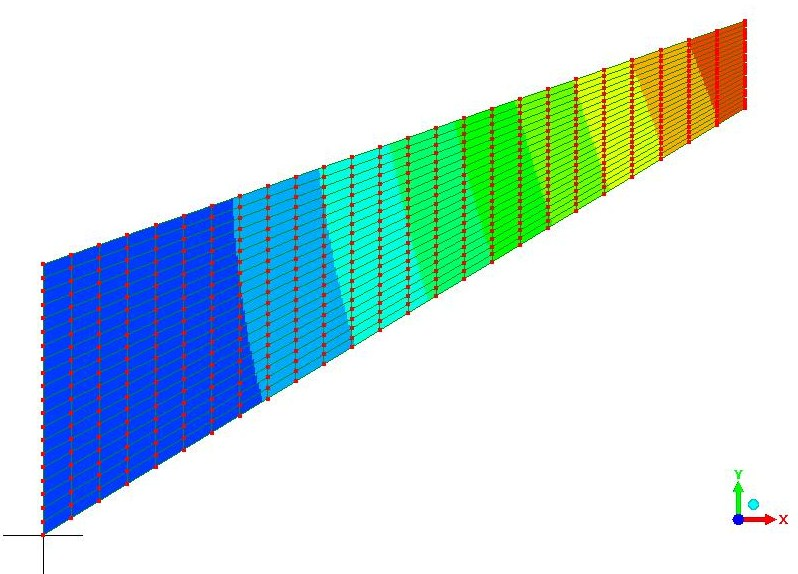
\includegraphics[width=0.49\textwidth]{schwingung1.jpg}}
   \hfill
   \subfigure[1. Harmonische \label{fig:schw1b}]
   {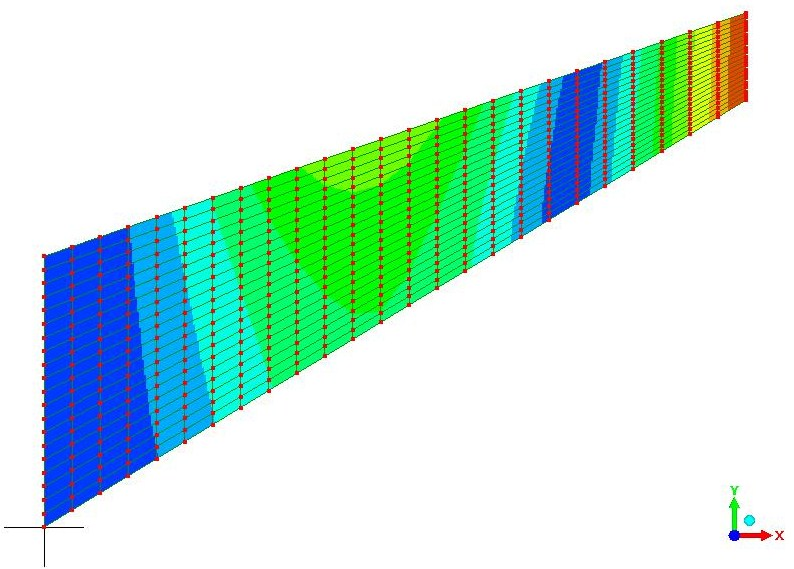
\includegraphics[width=0.49\textwidth]{schwingung1b}}
   \caption{Schwingungen, bei der sich die Spitze hoch und herunter bewegt}
   \label{fig:fspitze}
 \end{figure}

\begin{figure}[!htb]
	\centering
	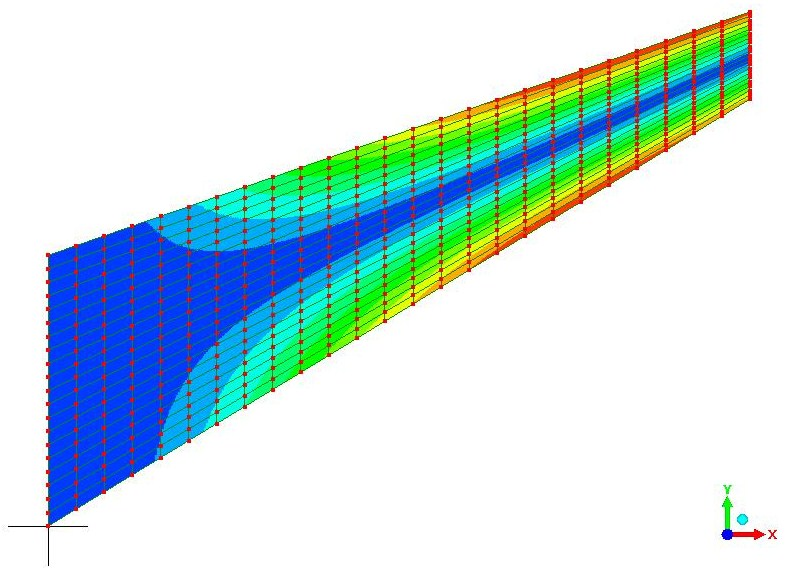
\includegraphics[width=0.8\textwidth]{schwingung2.jpg}
	\caption{Torsionsschwingung}
	\label{fig:torsion}
\end{figure}

\section{Weiteres}
Wir haben hier nur den Flügel untersucht.
Normalerweise muss man das ganze Flugzeug betrachten: So kann es zu komplexen Schwingungsformen kommen, bei der zB. das Höhenleitwerk mitschwingt, etc.
Außerdem kann man das Flugzeug im Windkanal testen, um auch noch die aerodynamischen Komponenten zu berücksichtigen.

\end{document}
